\chapter{Use case}

In this chapter we will outline our vision for both the application's user interface and its toolset.

\section{Wireframe of the application}\label{sec:wireframe}

Figure \ref{fig:wireframe} provides a simple wireframe sketch of the application graphical user interface (GUI). The window consists of several usual components:
\begin{itemize}
\item A horizontal toolbar at the top, allowing for a fast selection of tools and file manipulation
\item A 3D preview window, with live preview of the object. This window allows rotating and magnifying the object, as well as the application of selected tools (e.g. painting with a brush). A simple grid and a 3D cross is provided to ensure the user is always aware of object orientation, as it is important for 3D printing.
\item An options window on the right allows the user to customize the settings of the currently selected tool (e.g. selecting the color for a brush).
\end{itemize}

\hspace{-30pt}
\begin{figure}
	\centering
	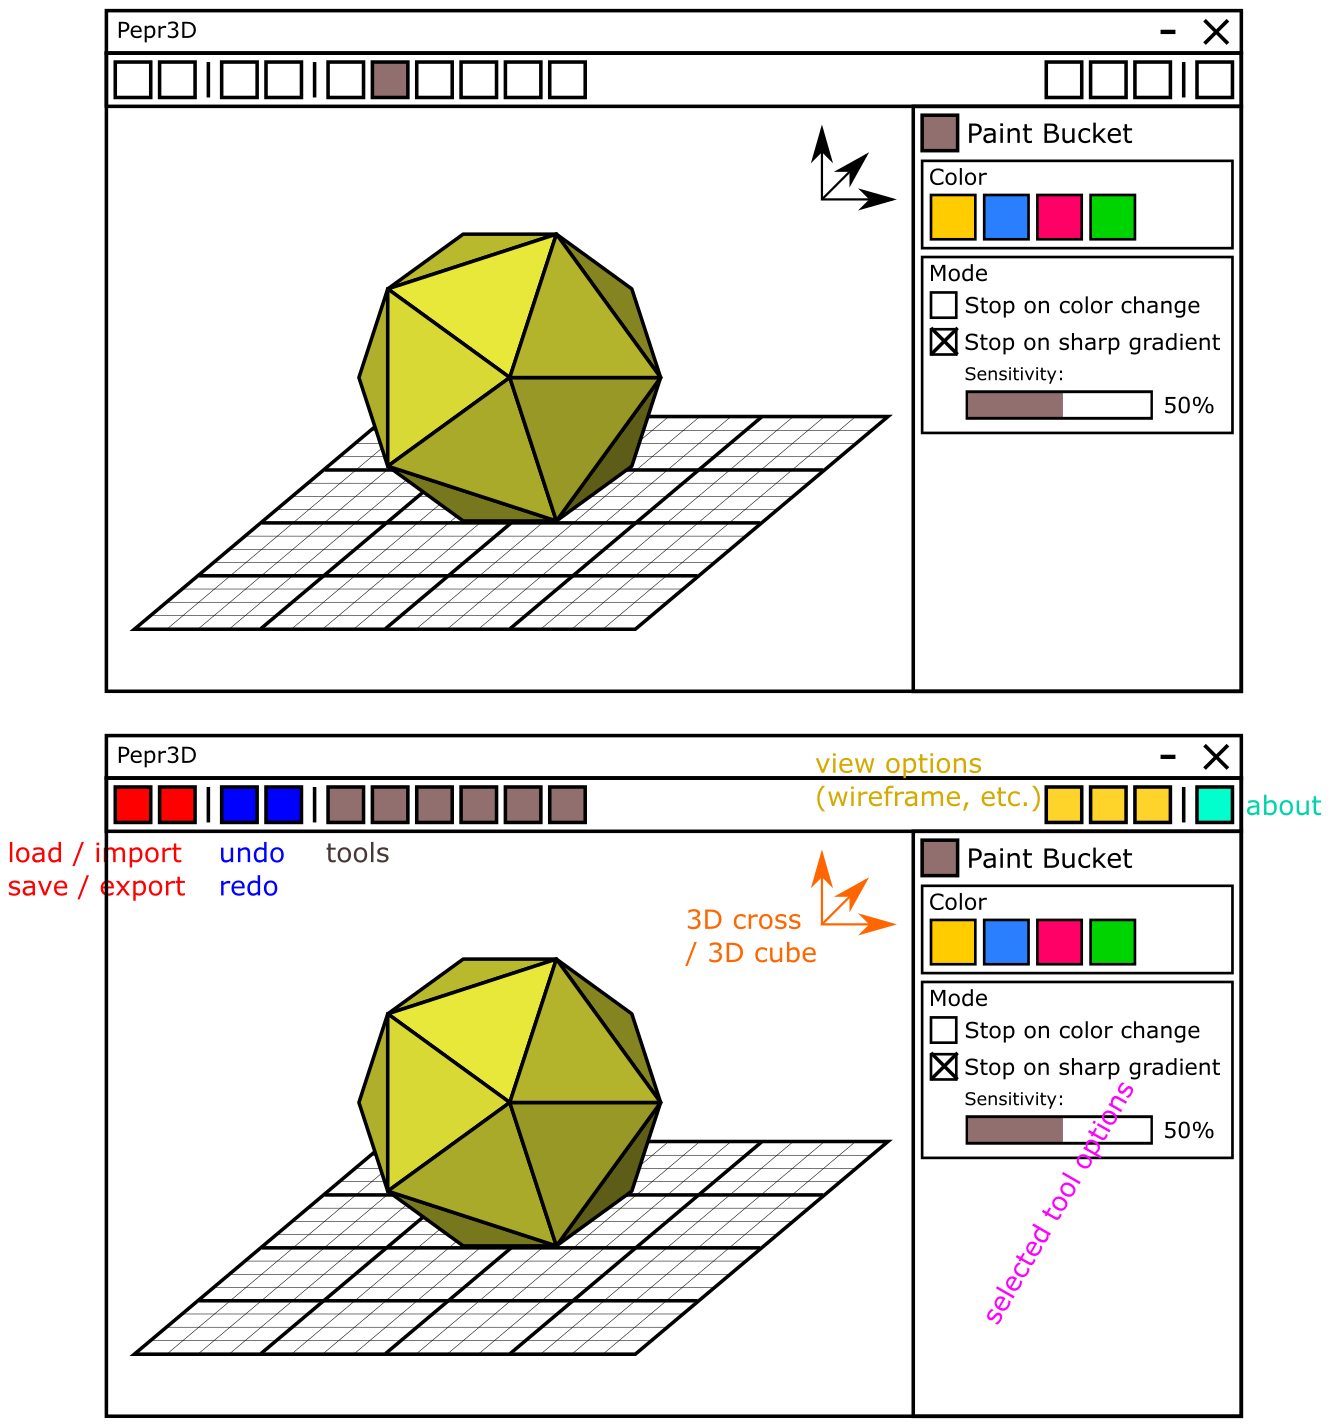
\includegraphics[scale=0.35]{images/wireframe.png}
	\caption{A simple wireframe sketch of the application.}
	\label{fig:wireframe}
\end{figure}

\section{Workflow and editor tools}

In this section we describe the intended workflow for a user who has a 3D model he wishes to color and then print on a multicolor FDM printer. This application is intended for users of varying degrees of experience and our goal is to create as easy-to-use application as possible.

\subsection{Importing the model}

First, the user has to import the model he found or created. Clicking on the \textit{import button} creates a dialog, the user selects the 3D model and the model gets loaded. The application should accept at least a few standard formats -- namely Wavefront $.$obj and $.$stl \footnote{https://en.wikipedia.org/wiki/STL\_(file\_format)}, both of which are widespread and well known among the 3D printing community.

The user should also be able to continue on an already existing project made earlier with Pepr3D.

After the model is loaded, it will be rendered in the 3D preview window. The window allows the user to rotate, zoom in and out and preview the wireframe of the model (rendering only edges and no faces of the model). The user is able to set the number of colors he wants to use (by default $4$ because current Prusa printers support up to four colors). The model is colored with the first color by default.

The user then selects one of the tools from the toolbar. This will bring up the \textit{Tool options} menu on the right hand side allowing the user to customize the tool.

Our application should support the \textit{Drag \& Drop} feature, so importing both the model and an already existing Pepr3D project is possible by dragging the file directly onto the viewport.

\subsection{Tools}

In this section we present the list of tools we think are best suited for our task. For each tool we provide the basic overview of its function, a simple reasoning why the tool is valuable for the user and a general sketch of the tool's properties.

\subsubsection{Edit history}
%TODO nafukovací feature
The user is always able to revert his last action by using an \textit{Undo button} or a keyboard shortcut. Depending on the technical difficulties, this feature could also persist through different sessions.

\subsubsection{Save as Pepr3D project}
Saves the current project as a Pepr3D project file. Upon re-opening Pepr3D, the user can load the project back and continue the work as if he never left. Does not include exporting the file into a slicer-compatible format.

\subsubsection{Export}
Export the file into a slicer-compatible format. This file is then handed to the slicing program (e.g. Slic3r Prusa Edition we mentioned earlier) and can be printed directly.

\subsubsection{Triangle painter}
After selecting a color, the user can assign said color to triangles he clicks on. Backside filtering is always on, so the user can only ever color a visible triangle, which should prevent a lot of accidents a lesser experienced user might make.

This is the simplest way to color the user's model and may be desirable as a quick way to correct any small errors made by either the user or the automatic segmentation itself. This tool also allows for very quick and easy coloring of very simple models (like a cube) that have a very low triangle count when the user wishes for a simple outcome -- for example a playing dice with six differently colored sides.

The \textit{properties} of this tool are very simple -- the user chooses a color to assign to the triangles that he clicks on. Depending on testing and remaining time, this tool could be expanded to include a radius and instead of coloring the single triangle the user clicks on, we could color all triangles in the vicinity of the clicked triangle instead.

\subsubsection{Bucket painting}
The user selects a color and by clicking anywhere on the model paints all triangles with selected color until an edge criterion is met. The simplest and most intuitive edge criterion is continuity (a hole stops the bucket spread). Several more criterions could be useful when in 3D, namely the sharpness of the normal (if two neighbouring triangles are at an angle greater than $X$, stop.) or a big gradient in a \textit{shape diameter function} (SDF).

A little more complex but a very intuitive tool that allows the user to get a quick initial paint on the model, which can later be adjusted with the Triangle painter tool, or made more complex with the finer Brush tool.

We already mentioned the main \textit{property} of the tool --- the edge criterion. A color-picker is, of course, necessary as well.

\subsubsection{Automatic segmentation}
Pepr3D fully automatically colors the whole model using the selected colors, according to a edge criterion as discussed in the \textit{Bucket painting} section. The user can then decide if he wants to merge some segments together, reducing the number of colors.

This tool should serve as a reliable way to color simple models which can be very distinctly separated into a number of regions, like a guitar which has two main parts -- the body and the neck.

The \textit{properties} of this tool are as following:
\begin{itemize}
\item The number of regions
\item The colors assigned to the regions
\item The edge criterion settings
\end{itemize}

\subsubsection{Semi-automatic segmentation}
The user roughly paints over triangles in areas that should have distinct colors, as indicated by Figure \ref{fig:rabbit}. The program then finishes the coloring by executing a clever flood-fill algorithm utilizing SDF, sharp edges, etc. 

\begin{figure}
	\centering
	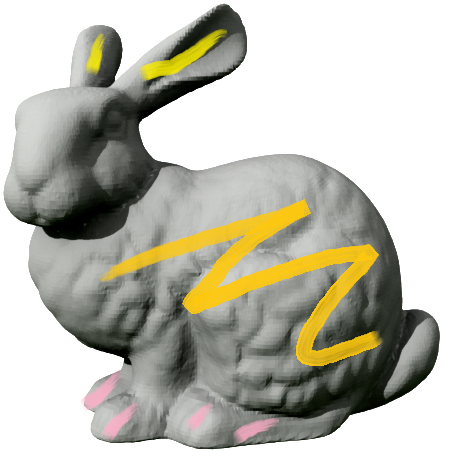
\includegraphics[scale=0.75]{images/rabbit.png}
	\caption{Semi-automatic segmentation as seen from the user's perspective. The ears of the rabbit are yellow as indicated by one stroke on each ear. The body is orange as indicated by the stroke on its back. The rabbit's feet are pink -- four pink strokes.}
	\label{fig:rabbit}
\end{figure}

This tool is primarily aimed at models that do not clearly separate into a few regions, and as such the computer would have a hard time guessing which regions the user had in mind. It is quick to use, since it requires non-precise brush strokes and should be a significant speed up when compared with just using the Bucket and Triangle painters to do all the work manually. Some manual adjustment is expected from the user but the main bulk of the painting should be done automatically.

The properties are very similar to automatic segmentation, the only exception being that the program will actually require the user to paint with the colors assigned to each region, after the user chooses the colors. If any of the brush strokes are missing, the program can either completely skip the color or generate the missing region automatically. The specific behavior will be chosen once both approaches are tested by the team.

\subsubsection{Brush}
A simple to use brush tool that allows to paint onto the model with a selected color. This tool allows the user to paint finer details, even though the geometry does not include them. For example painting the nose of the rabbit from Figure \ref{fig:rabbit} black -- there is no distinct edges on the nose, but the user can color only the nose by fine strokes of the brush.

The implementation of this tools is harder, because the program needs to adaptively subsample the triangle mesh to allow for finer details. This poses a lot of problems, which will later be discussed in the implementation parts of the document.

The \textit{properties} of the Brush tool include the color the user wishes to paint with, the shape of the brush itself and the size of the brush. A fail-safe setting that will stop subdividing triangles if they are smaller than the set number should be present, to avoid the user accidentally creating a model too complex for their computer to handle.

\subsubsection{Text}
Using the \textit{tool options} window, the user selects a font and types a custom text into a window. The text gets projected onto the model using some sort of projection transformation (customizable by the user from a limited range of projections). The software also allows extruding the projected text in the direction of the surface normal to create a $3$D effect.

We anticipate that this will be a very popular feature, especially among companies, since printing their own promotional items, with the ability to emboss the items with the company's name and logo seems very useful. 

The \textit{properties} of this tool include the standard feature-set of text editing -- the font, size, style (bold, italics, underlined, etc.) as well as the color of the letters. The more advanced settings of this tool include the projection type, and since we allow the extrusion of the text above the surface itself, the height will have to specified as well.

\subsubsection{Triangle subdivision/decimation}
The user selects a section of triangles and then presses either subdivide or decimate, which will either make the geometry more complicated, or more simple. See Figure \ref{fig:decimated} for visual aid. Please note that our tool is not a sculpting tool and such this tool might not allow the same extent of modifying the model as some 3D editors do.

\begin{figure}
	\centering
	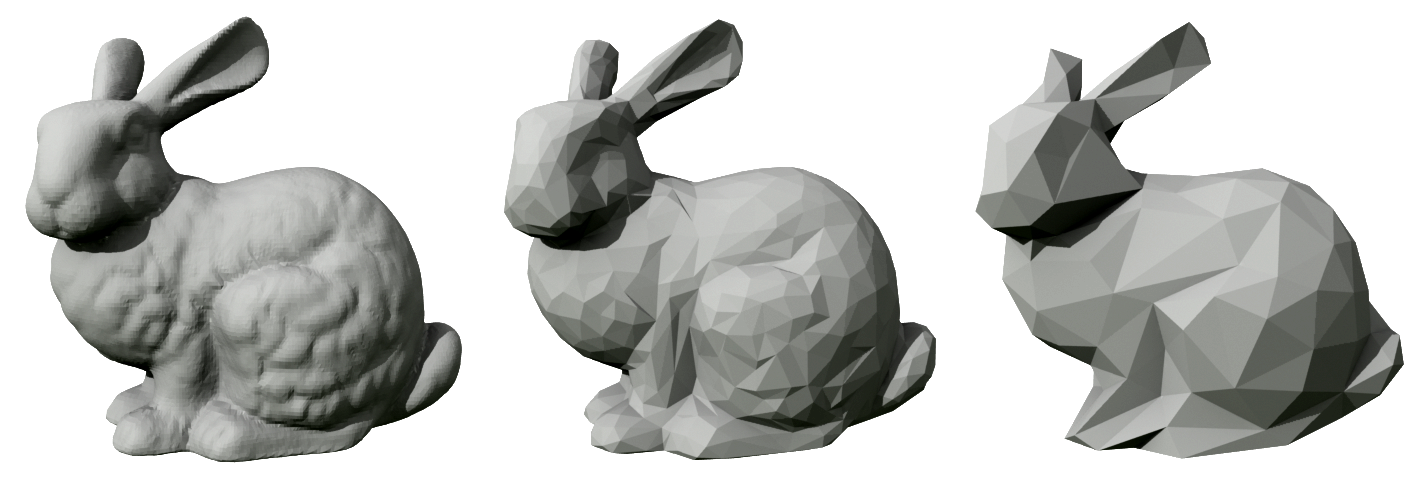
\includegraphics[scale=0.25]{images/decimated_bunny.png}
	\caption{Three stages of triangle numbers. The bunny on the left has the most triangles and most complicated geometry. Several decimations can reduce the number of triangles but also the number of details as shown on the second and third bunny.}
	\label{fig:decimated}
\end{figure}

We anticipate this to be a niche tool, used only by the more experienced users. We chose to include it, since it allows the professional printers to fine-tune their models for better performance or more precise coloring or printing.